\documentclass[12pt,twocolumn,a4paper]{article}
\usepackage[utf8]{inputenc}
\usepackage{amsmath}
\usepackage{amsfonts}
\usepackage{amssymb}
\usepackage{graphicx}
\usepackage{caption}
\usepackage{subcaption}
\usepackage{booktabs}
\usepackage{multirow} 


\usepackage[left=2cm,right=2cm,top=2cm,bottom=2cm]{geometry}


\title{ESTIMACIÓN DEL TAMAÑO Y LA VELOCIDAD DE
MICROBURBUJAS EN SISTEMAS DE FLOTACIÓN POR
AIRE DISUELTO, UTILIZANDO MICROFOTOGRAFÍA}
\author{Ordonez,Carlos;  Guerrero, Maria; España Elena;Florez, Juan 
 \\ 
\and{Universidad de Cauca, Popayán, Colombia.}\\
}

\begin{document}
\maketitle
\textbf{Resumen.}
La eficiencia de los sistemas DAF, tiene una estrecha relación con el diámetro y velocidad de las microburbujas, pero muchos de los medios para poder caracterizar las microburbujas requieren de adaptaciones al proceso y/o el uso de dispositivos de altas prestaciones, es por ello que en este proyecto se busca, el desarrollo de una aplicación para realizar esta caracterización, con la ayuda de un teléfono móvil. 

\textit{Abstract.}  
\textit{The efficiency of the DAF systems is closely related to the diameter and speed of the microbubbles, but many of the means to characterize the microbubbles require adaptations to the process and/or the use of high-performance devices, which is why In this project, the development of an application to carry out this characterization is sought, with the help of a mobile phone.}

\section{Introducción}

Las microburbujas son utilizadas en procesos industriales, que hacen uso de flotación por aire disuelto (DAF) \cite{cheng2016bubble}, para la clarificación de aguas y eliminación de residuos. Dentro de estos procesos la caracterización de las burbujas juega un papel importante, tanto en el rendimiento \cite{gulden2018online} \cite{eskanlou2018interactional} \cite{reis2016study}, como en la eficiencia de la limpieza de aguas \cite{sadeghi2020experimental} \cite{fanaie2020effect}. El tamaño de las microburbujas puede verse afectado en el ascenso de las misma debido a la coalescencia con otras burbujas \cite{fanaie2020effect}, el diámetro de la burbuja afecta la capacidad para eliminar partículas \cite{sadeghi2020experimental}, las burbujas de mayor tamaño suben con una velocidad superior capturando partículas más grandes, mientras que las pequeñas tiene una velocidad de ascenso más baja y recolectan partículas de menor dimensión \cite{sadeghi2020experimental} \cite{brasileiro2020construction}, es por ello que es importante caracterizar las burbujas o microburbujas en cada proceso \cite{sadeghi2020experimental} \cite{ahmadi2014nano}.


Idealmente, la caracterización de microburbujas debe presentar una mínima interferencia en el comportamiento dinámico de estas, ya sea en su tamaño o en su velocidad de ascenso \cite{gulden2018online}. El análisis de microburbujas debe poseer las características necesarias para lograr una operación en línea  bajo condiciones variables en su entorno de operación, las variables dinámicas de las burbujas requieren ser analizadas de forma precisa \cite{parmar2015terminal}, sin comprometer el proceso DAF a adaptaciones complejas y que pueda ser utilizado en distintas plantas que usen flotación por aire disuelto con aguas a tratar.

Es fácil captar una burbuja ascendente y determinar sus características dinámicas, pero al  analizar cúmulos de microburbujas en diferentes condiciones del fluido a tratar, se hace necesario la adaptación de sensores y dispositivos para lograr esta tarea \cite{brasileiro2020construction}. Existen diferentes métodos para la caracterización de microburbujas, como: análisis de imagen \cite{swart2020situ}, microfotografía \cite{sadeghi2020experimental}, acústico \cite{guan2017bubble}, Velocimetria de partículas \cite{levitsky2021microbubbles}, difracción láser \cite{reis2016study}, desacople de gases \cite{parmar2015terminal}, aunque en su mayoría presentan buenos resultados en la caracterización \cite{gulden2018online} \cite{eskanlou2018interactional} \cite{aumelas2016micro}, gran parte de la implementación de estos métodos incurre en tecnologías o adaptaciones complejas y costosas, las cuales generalmente utilizan columnas, tubos o celdas paralelas al proceso \cite{reis2016study}  \cite{swart2020situ}  \cite{han2002development}, \cite{cheng2016bubble}, \cite{jeon2018bubble}, estas causan que las microburbujas sean más sensibles a los ajustes de los instrumentos \cite{jeon2018bubble}, lo que complica el buen análisis de las microburbujas.

Los avances en teléfonos inteligentes, en especial la capacidad de grabar vídeo en cámara lenta, alta resolución de imagen, la diversidad de aditamentos para captura de imágenes, los hace atractivos para su uso en aplicaciones de microfotografía. En particular, porque es un dispositivo que necesita pocos recursos para esta tarea, presenta una flexibilidad en su uso dentro y fuera del laboratorio \cite{orth2018dual}. Es por ello que se propone el diseñar e implementación de un sistema de microfotografía que use un teléfono inteligente con buenas características de toma de imagenes para determinar el tamaño y velocidad de microburbujas, sin usar columna de flotación independiente, directamente   en el prototipo de la planta de DAF instalado en el laboratorio de hidráulica de la Universidad de Cauca.

El artículo se compone de 5 secciones, en la sección l se encuentra la introducción, En la sección II se encuentra la metodología, en la sección III  se presentan los resultados,  en la sección IV  conclusiones.

\section{Metodología}
La metodología a seguir para la implementación de la propuesta, está dividido en 3 fases, primera fase correspondiente al diseño del sistema de microfotografía,  la segunda enfocada en el desarrollo del algoritmo basado en visión de máquina, finalmente se describe el proceso de toma de vídeos para su posterior procesamiento.
\subsection{Sistema de Microfotografía}

Debido a las características particulares presentes en la planta en la cual se pondrá a prueba el sistema de microfotografía, se selecciono los siguientes elementos que permiten cumplir la labor de caracterización de microburbujas de formas más cómoda y eficiente. Como soporte se creó una base de aluminio, la cual  se compone de dos ganchos los cuales se ajustan en la parte superior de un lateral del tanque DAF y la base donde se acomoda la cámara como se muestra en la figura \ref{soporte}, este permite que la cámara se encuentre lo más cerca al tanque, logrando así una mejor captura de las microburbujas, la base cuenta con unas medidas de 4*17*1 cm de alto, ancho y profundidad respectivamente, y los ganchos o brazos tienen   30*1*0,2 cm de alto, ancho y profundidad, una distancia de doblez  de 3,5 cm,  en esta última medida se tuvo en cuenta el tamaño del lente y el de la propia base, ajustando de forma precisa el montaje de microfotografía evitando así interferir en el ángulo de la cámara \cite{tripode}. 

\begin{figure}[h]
	\centering
	\includegraphics[scale=0.5]{soporte.png}
	\caption{Soporte para teléfono móvil} \textbf{Fuente:} Elaboración propia
	\label{soporte}
\end{figure}

Como sistema de iluminación, se emplea una sola fuente de  luz  ubicada en el lado opuesto de la  cámara generando con ello una sistema de luz de fondo, se eligió una lámpara de panel led  cuadrado S/p luz dia marca Karluz como se muestra en la figura \ref{lampara}, referencia kl-2201, con un Voltaje de 110 V  y una potencia de 12 W \cite{lampara} 

\begin{figure}[h]
	\centering
	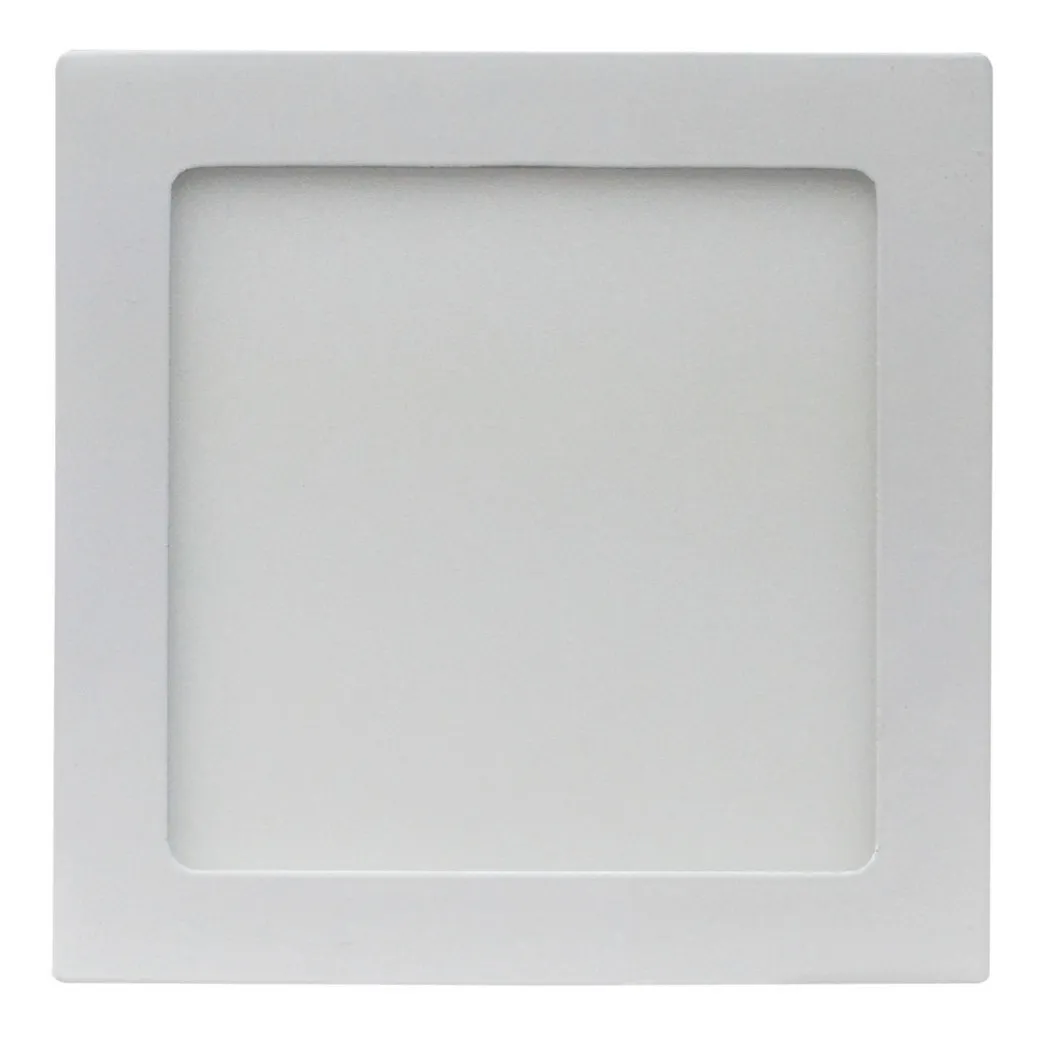
\includegraphics[scale=0.2]{lampara.jpg}
	\caption{Lámpara de 12 W} \textbf{Tomado:} \cite{lampara}
	\label{lampara}
\end{figure}

El mecanismo óptico a utilizar es un "Lente Gran Angular" para teléfono inteligente como se muestra en la figura \ref{lente}, con clip 2 en 1,  compatible con iPhone, Samsung, Google Pixel, tiene unas dimensiones de 11.5cm*10.3cm*5.9cm, minimiza el deslumbramiento de la lente, la reflexión, el fantasma y otros artefactos para una excelente claridad,  dentro de sus características cuenta con un distancia focal de aproximadamente 7 cm permitiendo así una captura óptima de la imagen, Lente macro de 12,5 x,  lente de rosca de 1.457 pulgadas de diámetro, permite tomar fotos a una distancia de 1.18 a 1.57 pulgadas \cite{lente}. Este estará ubicado sobre el lente de la cámara.

\begin{figure}[h]
	\centering
	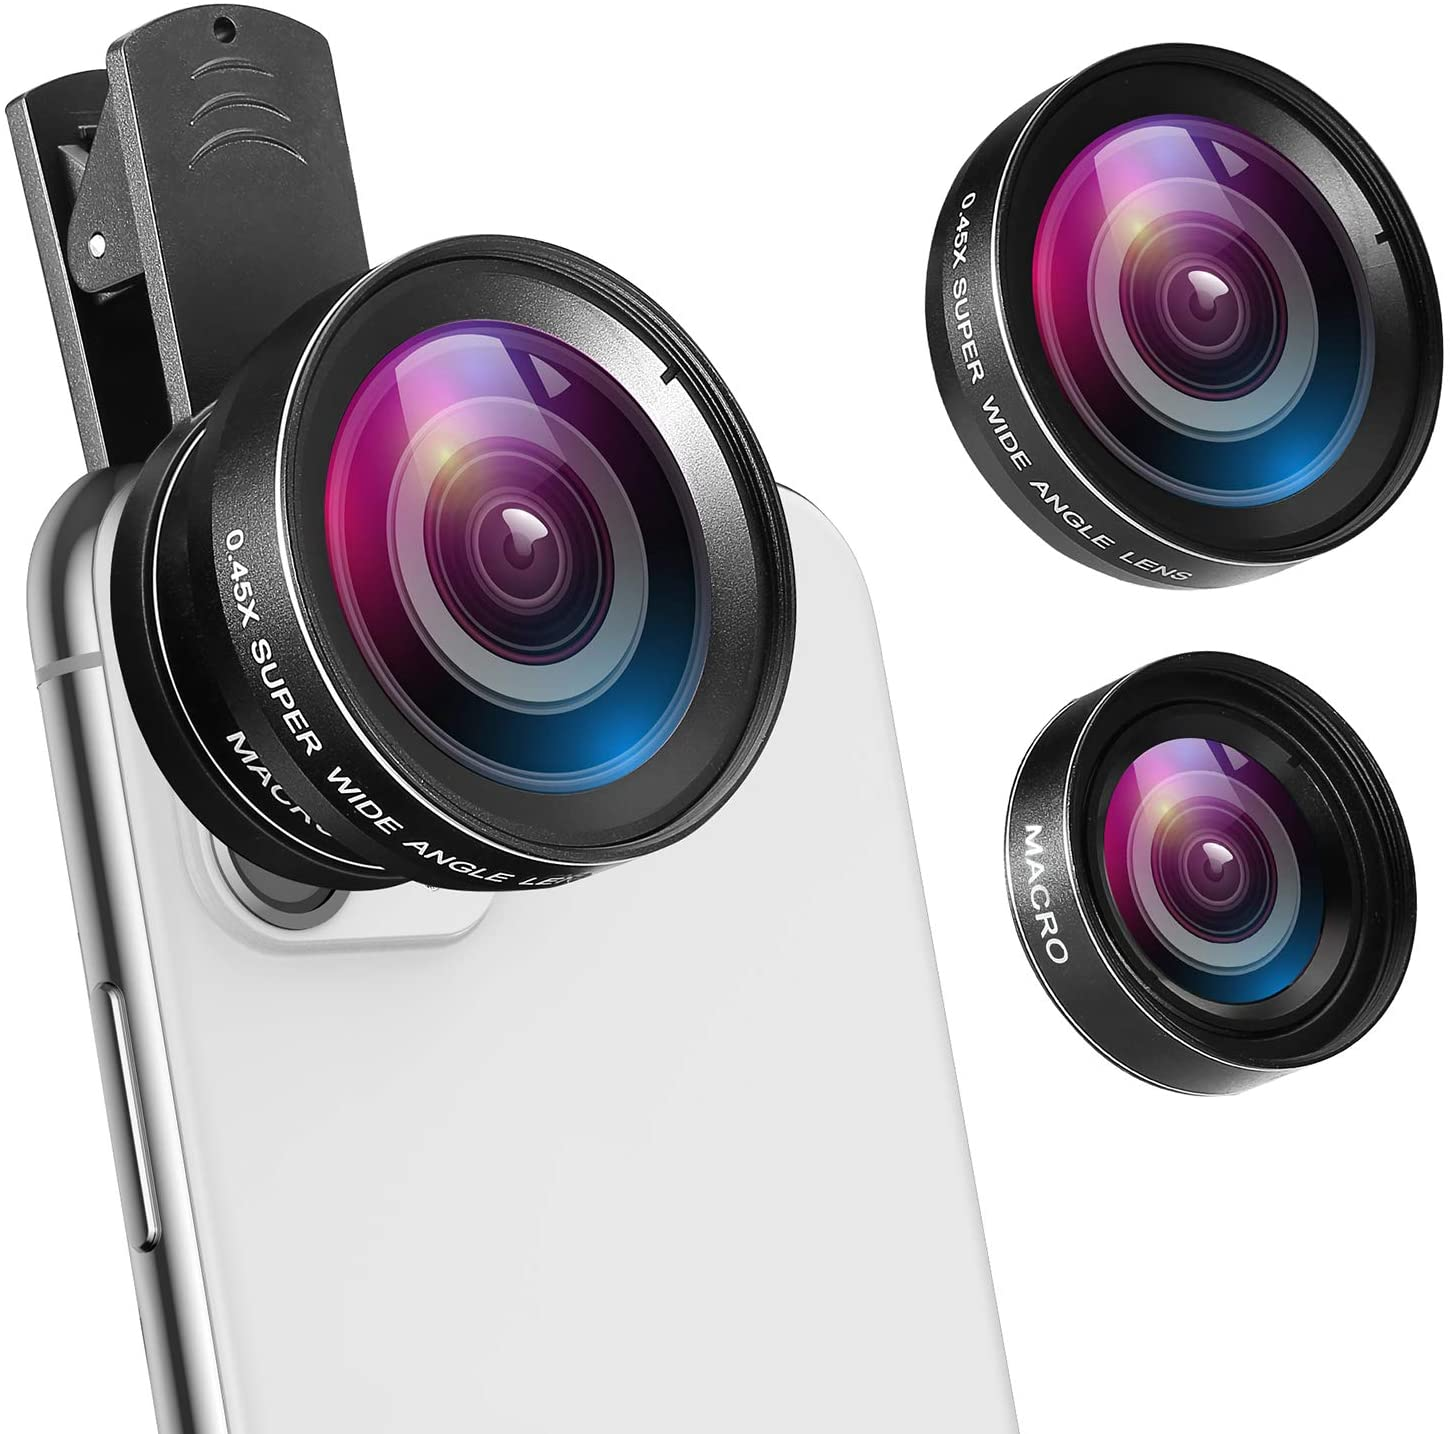
\includegraphics[scale=0.1]{lente.jpg}
	\caption{Lente para teléfono inteligente} \textbf{Tomado:} \cite{lente}
	\label{lente}
\end{figure}

La cámara a utilizar es de un teléfono inteligente Huawei P30 pro, con 4 cámaras un lente SuperZoom, y un  lente ultra gran angular de 20 MP, la cámara es Super Sensing de 40 MP con un Zoom de 50x, la cámara posterior, es compatible con el enfoque automático (enfoque láser, enfoque de fase, enfoque de contraste), es compatible con AIS (Estabilización de imagen con IA de HUAWEI), cabe resaltar que en diferentes modos de fotografía, el número de píxeles puede ser ligeramente diferente \ref{hawei}, dentro de los detalles más relevantes de la cámara se encuentra:

\begin{itemize}
\item CÁMARA POSTERIOR: Cámara cuádruple Leica: 40 MP (objetivo gran angular, apertura de f/1.6, OIS) + 20MPX (objetivo ultra gran angular, apertura de f/2.2) + 8 MP (teleobjetivo, apertura de f/3.4, OIS) la cámara de tiempo de vuelo (Time-of-Flight, TOF).
\item CÁMARA FRONTAL: 32 MP, apertura de f/2.0.
\item CAPTURA DE VÍDEO: en cámara lenta de hasta 960 fps (velocidad X32).
\end{itemize}


\begin{figure}[h]
	\centering
	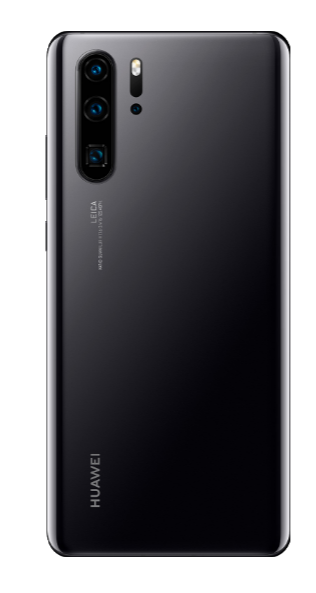
\includegraphics[scale=0.3]{hawei.png}
	\caption{Teléfono inteligente} \textbf{Tomado:} \cite{Hawei} 
	\label{hawei}
\end{figure}

Estos elementos se acoplan al sistema DAF,como se muestra en la figura \ref{disDAF}.

\begin{figure}[h]
	\centering
	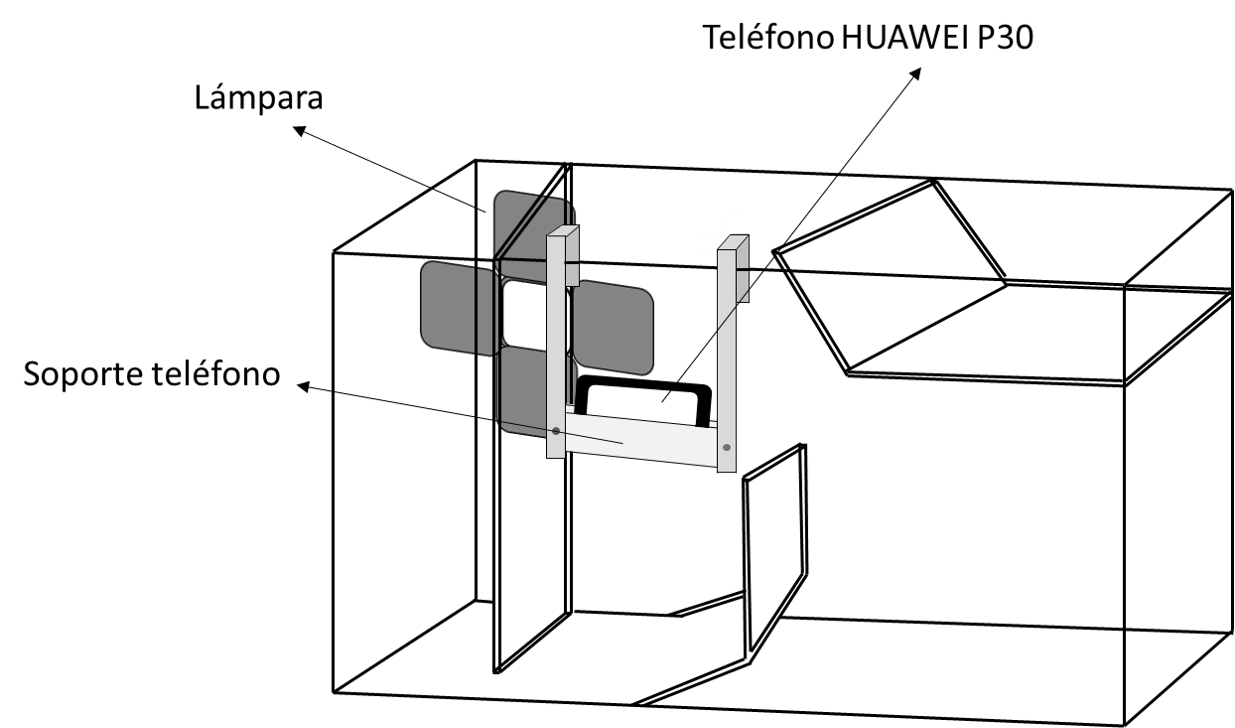
\includegraphics[scale=0.3]{Distribucion2.png}
	\caption{Distribución de los componentes de microfotografía en el sistema DAF} \textbf{Fuente:} Elaboración propia
	\label{disDAF}
\end{figure}

\subsection{Software}
El algoritmo se realizo en C\#, en la plataforma unity, con ayuda de la librería de uso libre OpenCV versión 1.7.1.

Esta sección estará dividida en 5 secciones, la primera enfocada en la preparación del vídeo, pre-procesamiento;  la segunda, es  el procesamiento inicial que se le aplicará al vídeo obtenido anteriormente con le fin de eliminar el mayor ruido posible, la siguiente en donde se explica el proceso de detección de las microburbujas en frames de vídeo, la cuarta  en donde se describe el proceso utilizado para realizar el seguimiento de las MB detectadas, en la última parte se encuentra el proceso de caracterización.

\subsubsection{Pre-procesamiento de vídeo}

El vídeo que procesa el algoritmo, se encuentra en formato 3D, es por ello que se realiza un paso a formato 2D, al igual que transformaciones para que cada frame del vídeo, pase por los distintos filtros. 

\subsubsection{Eliminación de ruido}
Para el proceso de caracterización, es importante que el objeto sea fácil de diferenciar del fondo, es por ello que se hace uso de los siguientes filtros.

\begin{enumerate}
\item Conversión a escala de grises, con el objetivo de evitar reflejos indeseados. 
\item Filtro de mediana, con la finalidad de eliminar contrastes de color fuertes.
\item Filtro de Gauss, para difuminar los elementos irrelevantes y el ruido
\item Operaciones morfológicas, con el fin de mejorar la calidad del objeto a inspeccionar.
\item Filtro de Canny, con el propósito de realzar el contorno de las microburbujas.
\end{enumerate}

Es de resaltar, la aplicación será en el orden expuesto. 


\subsubsection{Detección de microburbujas}

Para realizar la identificación de MB, se utilizó la transformada de Hough, esta función retorna un arreglo, de lo que en C\# denomina CircleSegment, que contiene la información de radio, posición en $x$, $y$; de cada microburbuja que se detectó, que es almacenada para un uso posterior, además se guardó, la información de las burbujas que llegan desde abajo, evitando con ello hacer seguimiento de las que provengan en otras direcciones y puedan entorpecer el proceso de caracterización. 


\subsubsection{Calculo de trayectorias}

Para iniciar con el algoritmo de seguimiento, el cual se encarga de identificar una misma burbuja a lo largo de la trayectoria, hay que tener presente que el ascenso de las burbujas no es lineal, por lo que para el cálculo de distancia se usa la forma euclidiana, además se hace necesario declarar un listado auxiliar en donde se almacenarán las burbujas ya ordenadas de acuerdo a su par anterior; del proceso anterior se retornan dos listas que contienen el radio, la coordenada en $x$ y la coordenada en $y$, de las burbujas que llegan desde abajo y las burbujas totales en el frame,  para iniciar el proceso se hace un recorrido de cada uno de los elementos guardados en la lista de burbujas que llegan desde abajo, y a este se le aplica la función de distancias mínimas, la cual consiste en declarar un lista de coordenadas de distancias inicialmente vacía, se toma cada valor de la MB que viene desde abajo y por cada burbuja detectada se calcula la distancia, es decir, se tiene el  punto $x(1)$, y $x(2)$ para calcular la distancia en $x$, además de $y(1)$ y $y(2)$ para calcular la distancia en $Y$, con los dos valores se aplica la raíz cuadrada de la suma de los cuadrados,  obteniendo así la distancia para cada burbuja y se almacena en un la lista de distancias, como lo que se busca es las coordenadas de la burbuja para futuros procesos y se sabe que la posición de las coordenadas corresponde al de la distancia, pero el valor de interés es el más pequeño, entonces se creó una lista copia de las distancias, a la cual se le realizó un ordenamiento y con ello se obtiene que en la posición 0 esta la distancia más pequeña, ya con el valor de distancia mínima determinada, se busca la posición de esta distancia en la lista original, con la ubicación encontrada, se procede a guardar las coordenadas de la burbuja en la lista MB ordenadas.

\subsubsection{Calculo de diámetro y velocidad }

Este algoritmo recibe las burbujas ordenadas que serían las actuales, y por cada burbuja calcula la velocidad, pero para calcular la velocidad es necesario tener la distancia recorrida, se puede obtener a través de la fórmula euclidiana, para ello se hace uso de una variable auxiliar que permite recorrer la lista de coordenadas anteriores, de forma paralela al recorrido de las actuales, con ello se tiene el  punto $x(1)$, y $x(2)$ para calcular la distancia en $x$, además de $y(1)$ y $y(2)$ para calcular la distancia en $y$, con los dos valores se aplica la raíz cuadrada de la suma de los cuadrados obteniendo así la distancia para cada burbuja, ahora falta dividir por el tiempo, que corresponde al tiempo del vídeo y multiplicar por el valor de conversión de pixeles a mm, el resultado es la velocidad en mm/seg.


\subsection{Adquisición de datos}

El propósito del proyecto es realizar el análisis de miroburbujas, a través de microfotografía, es por ello que se acopla el lente zoom, a la cámara del teléfono celular, este se ajusta al soporte para mantenerlo estático y minimizar el ruido.

Para iniciar la grabación de las microburbujas, se requiere establecer una conexión inalámbrica entre el teléfono celular y el computador, evitando así que el factor humano interfiera  con movimientos de la cámara, desconfiguraciones, entre otras; después de realizar con éxito la conexión,  se selecciona el modo de captura en “cámara lenta” y se desactiva el reconocimiento de movimiento, se debe configurar el modo de foco en manual, con el propósito de que el autoenfoque no vaya cambiando entre las cámaras del teléfono, también se configura el zoom a x2, los parámetros ISO, la apertura y la obturación según como se presenten las condiciones del entorno, esto refiere al posicionamiento del acople, ubicación de la lámpara y estado del tanque, manteniendo así un estándar para realizar este procedimiento.

En el control de iluminación, se hace cierre de las cortinas del laboratorio evitando así el ingreso de luz exterior, también se apagan las lámparas, dejando únicamente encendida la lámpara que está asociada al tanque DAF. Para posicionar la cámara, 
se utiliza el acople mencionado en la sección de diseño metodología, sistema de microfotografía, soporte para teléfono móvil, el cual se ubica al ras del tanque.



\section{Resultados}

En la realización de este proyecto se planteo la toma de videos a cámara lenta de la planta en funcionamiento a distintas presiones, las presiones que se escogieron fueron 34 y 36 psi, todo estos considerando el entorno y las limitaciones de la planta DAF del laboratorio de hidráulica de la Universidad del Cauca, se capturaran entre 10 a 27 videos con una duración de 10 segundos (tiempo es delimitado por el software de captura) por presión en cada prueba, realizando un total de 2 lotes de videos.

Ambas pruebas se realizaron bajo las siguientes condiciones: caudal de recirculación 1000 L/h y una inyección de aire de 0.1 L/m, la iluminación se mantuvo constante durante el proceso de realización del material multimedia, con la diferencia que cada lote hace uso de un distinto tubo Venturi, ya que al ser una impresión 3D la cavitación desgasta el material haciendo que algunas burbujas salgan con un tamaño relativamente más grande y también se debe tener en cuenta que cada tubo tendrá un comportamiento distinto al generar microburbujas ya que la impresión no son exacatamente iguales una de otras. 

En el primer lote se tomaron 18 videos con una presión de 34 psi y 22 videos con 36 psi, para un total de 40 videos, del total se seleccionaron 27 videos que cumplían las condiciones para ser procesados adecuadamente, estas condiciones radican en que el video presenten como minimo 10 microburbujas en el plano focal de la cámara. Los resultados obtenidos con las condiciones antes mencionadas y a una presión de 34  en cuanto a velocidad se presentan en la tabla \ref{R1}.

\begin{table*}[t]
	\begin{tabular}{| c | c | c | c | c | c | c | c |}
	\hline
	
		\multicolumn{8}{ |c| }{\textbf{Primer lote 34 psi}} \\ \hline
	 	\multirow{2}{*}{\textbf{Video}} & \multirow{2}{*}{\textbf{Burbujas}} & \multicolumn{3}{ |c| }{\textbf{Diametro ($\mu$m)}} & \multicolumn{3}{ |c| }{\textbf{Velocidad (mm/s)}} \\
 		&  & \textbf{Minimo} & \textbf{Maximo} & \textbf{Promedio} &\textbf{Minima} & \textbf{Maxima} & \textbf{Promedio}\\ \hline
 	1 & 17 & 52,8355 & 92,4621 & 72,24 & 2,0966 & 11,5869 & 2,65 \\
 	2 & 11 & 35,2236 & 88,0591 & 68,27 & 2,0966 & 5,3202 & 2,59 \\
 	3 & 19 & 22,0147 & 83,6562 & 49,23 & 2,0966 & 11,5869 & 2,65  \\
 	4 & 12 & 22,0147 & 105,6710 & 62,97 & 2,0966 & 7,8789 & 2,27  \\
 	5 & 14 & 22,0147 & 88,0591 & 47,12 & 2,0966 & 3,7016 & 2,17 \\
 	6 & 16 & 30,8207 & 118,8798 & 64,9 & 2,0966 & 11,0534 & 3,89 \\
 	7 & 16 & 26,4177 & 149,7005 & 104,63 & 2,0966 & 11,7166 & 2,32  \\
 	8 & 16 & 26,4177 & 70,4473 & 47,88 & 2,0966 & 2,0966 & 2,1 \\
 	9 & 16 & 26,4177 & 96,8650 & 62,52 & 2,0966 & 15,6273 & 7,71 \\
 	10 & 22 & 44,0295  & 118,8798 & 75,99 & 2,0966  & 5,8311 & 2,47 \\
 	11 & 10 & 22,0147  & 149,7005 & 52 & 2,0966  & 17,1599 & 3,55 \\
 	12 & 16 & 22,0147  & 134,7305 & 41,94 & 2,0966  & 14,8250 & 8,97 \\
 	13 & 13 & 22,0147 & 145,2976 & 61,31 & 2,0966 & 10,7277 & 3,6 \\
 	\bottomrule
	\end{tabular}
	\caption{Resultados primer lote 34 psi}
\label{R1}
\end{table*}

En el segundo lote, al igual que el primero se conservaron las condiciones previamente establecidas, con la única variante que para este lote se usó un distinto tubo Venturi, debido al desgaste antes mencionado, se tomaron 25 videos a 34 psi y para 36 psi 26 para un total de 41. De este lote se seleccionaron 24 videos que cumplían las condiciones antes expuestas, Los datos correspondientes a los resultados a una presión de 36psi del primer lote y los del segundo lote se encuentran en la sección de Anexos en las tablas \ref{R2}, \ref{R3} y \ref{R4} .

A partir de los datos presentados en las tablas, existió una distribución variada de tamaños de microburbujas cómo se expresa en el gráfico de la figura \ref{dispdia}, se puede apreciar rangos desde  22$\mu$m hasta 215$\mu$m aproximadamente, esto debido al desgaste mencionado del tubo Venturi a lo largo de su uso, pero esta situación dio oportunidades de presenciar distintos tamaños de burbujas para probar el alcance del algoritmo, el cual cumple satisfactoriamente la detección de burbujas dentro de los rangos estipulados en los objetivos e incluso tamaños mucho menores.

\begin{figure}[h!]
	\centering
	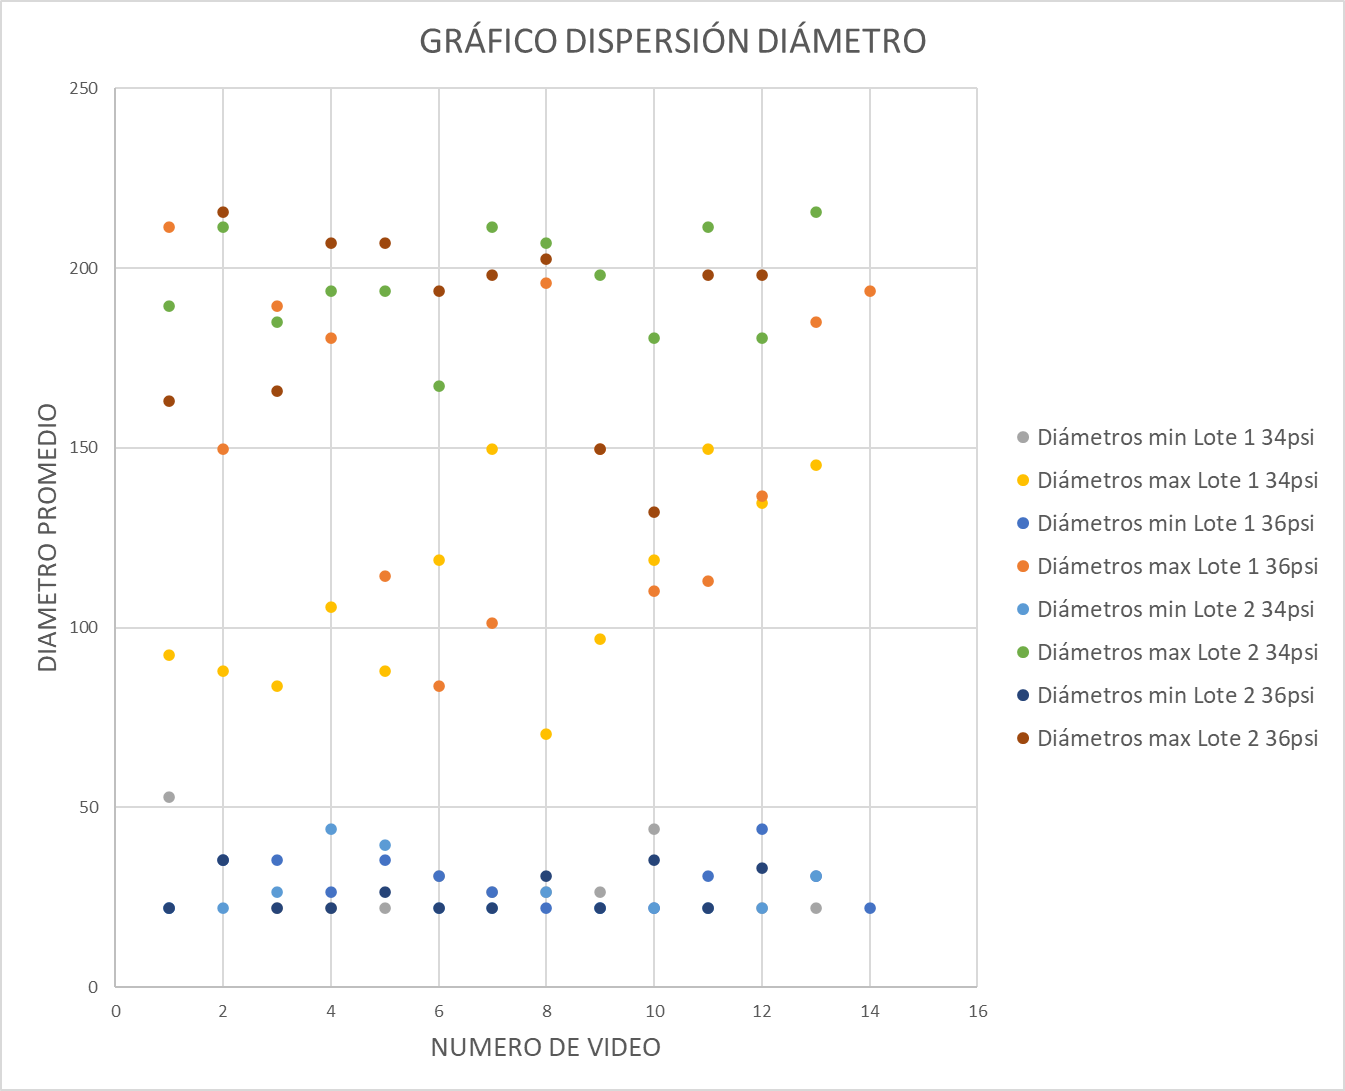
\includegraphics[scale=0.35]{dispDia.png}
	\caption{Dispersión de datos respecto al diámetro en ambas pruebas} \textbf{Referencia: Elaboración propia} 
	\label{dispdia}
\end{figure}
 
De la prueba también se observó que el promedio general en cuanto al  diámetro, los vídeos a 34psi del primer lote fue de 62,384$\mu$m y de 36 psi del mismo lote fue 76,24$\mu$m, por otro lado, en el segundo lote los promedios fueron de 80,6741667$\mu$m y 89,0792308$\mu$m para 36 y 34 psi respectivamente esta información se visualiza de mejor forma en las figuras \ref{diapro34} y \ref{diapro36}. Esta distinción en cuanto al tamaño promedio en cada lote se atribuye al cambio de tubos Venturi, puesto que al ser una impresión 3D, cada tubo presenta comportamientos distintos al generar microburbujas

\begin{figure}[h!]
	\centering
	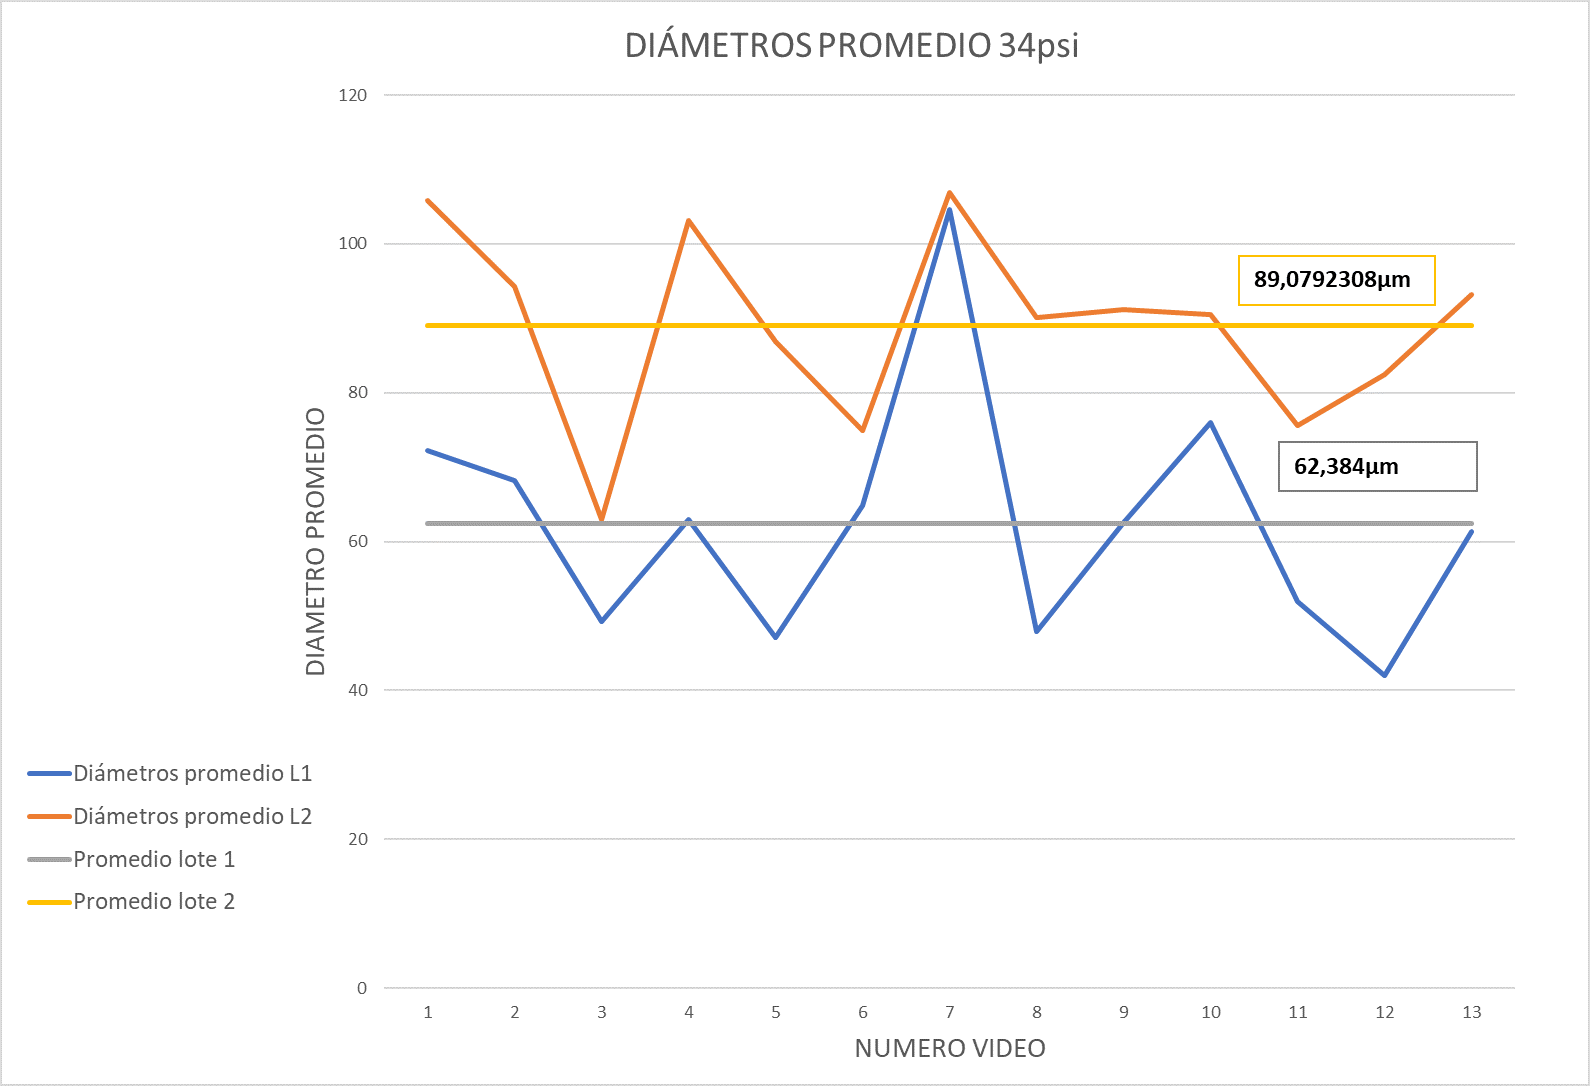
\includegraphics[scale=0.3]{Diapro34.png}
	\caption{Gráfico de tendencia de diámetro en ambos lotes 34 psi.} \textbf{Referencia: Elaboración propia} 
	\label{diapro34}
\end{figure}

\begin{figure}[h!]
	\centering
	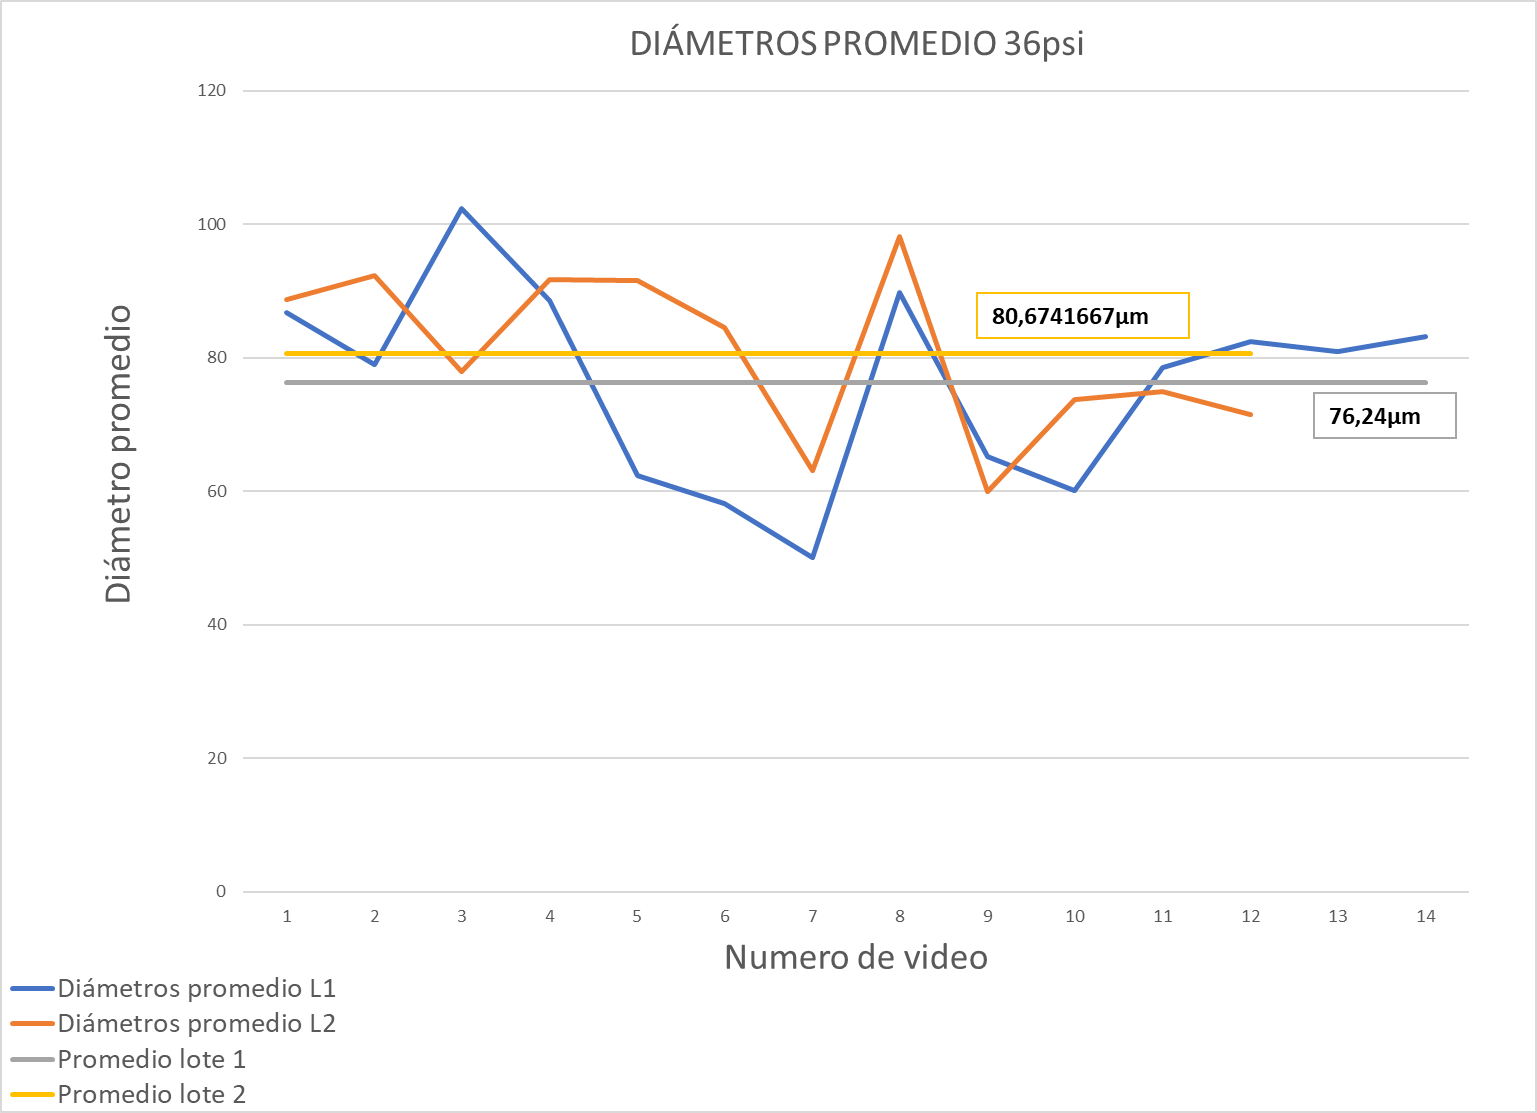
\includegraphics[scale=0.3]{Diapro36.png}
	\caption{Gráfico de tendencia de diámetro en ambos lotes 36 psi.} \textbf{Referencia: Elaboración propia} 
	\label{diapro36}
\end{figure}

En cuanto a la velocidad siempre se mantuvo un valor mínimo estable de 2,0966 mm/seg como se aprecia en la figura \ref{dispvel}, esto puesto a que la velocidad es influencia por el tamaño y que el algoritmo tiene un rango mínimo de detección por tamaño, las velocidades de estas pequeñas burbujas se mantenían prácticamente similares. Se presentó un rango de velocidad de 2,0966mm/seg hasta 21,8404 mm/seg, en el calculo de esta variable se presentaron algunos casos como que algunas burbujas presentaban una alta velocidad debido a que estas se estaban desplazando linealmente hacia arriba y también que algunas presentaban mayor tamaño, como la literatura define que burbujas de mayor tamaño tienen mayores velocidades, otro caso es el que algunas se desplazan hacia el fondo, lo cual da un efecto de velocidad mas reducida, Para comprobar esta cuestión se realizo un grafico donde se pintaba en tiempo real en la misma imagen la trayectoria de las burbujas dando una visualización del movimiento que estas hacían a lo largo del video como se muestra en la figura \ref{trayectoria}. En general las velocidades obtenidas entran dentro de los rangos estipulados en los objetivos e incluso el algoritmo es capaz de estimar velocidades mayores.

\begin{figure}[h!]
	\centering
	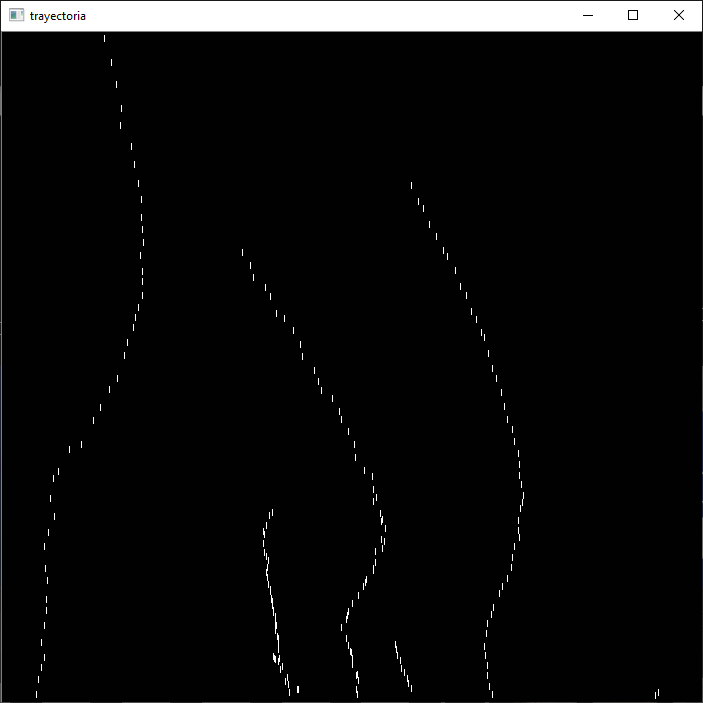
\includegraphics[scale=0.4]{trayectoria.png}
	\caption{Trayectoria del desplazamiento de las microburbujas } \textbf{Referencia: Elaboración propia} 
	\label{trayectoria}
\end{figure}

\begin{figure}[h!]

	\centering
	\includegraphics[scale=0.4]{Dispvel.png}
	\caption{Dispersión de datos respecto a la velocidad en ambas pruebas } \textbf{Referencia: Elaboración propia} 
	\label{dispvel}
\end{figure}

\section{Prueba Interfaz}

Una vez obtenido los vídeos y analizados, se procedió reuniendo un grupo de 24 personas, a las cuales se les dio un contexto del proyecto, se les compartió la aplicación y se los dejo interactuar con la misma por 10 min, en donde se resolvieron preguntas que fueron surgiendo a lo largo del proceso.

Después de compartirles la apk, se válido a que personas no les funcionó la aplicación, es decir  la aplicación no abría o se cerraba forzadamente, el 16.67\%, al igual que a los que les funcionaba la aplicación pero se ponía lenta o el vídeo no era fluido, el 25\% y por supuesto a las personas que les funcionó correctamente 58.33\%; también se les pidió que nos proporcionarán información sobre sus dispositivos como por ejemplo, Ram, Android, Procesador, de donde se obtuvo la siguiente información.



En la tabla \ref{TablaCEL}, en la sección de anexos, se  encuentra el resumen de la información recolectada, dejando solo las características únicas, para así poder saber  que referencias mínimas podría tener el teléfono, para realizar un correcto procesamiento de la información: se puede decir que los celular con ram menor de 4 GB no son capaces de correr la aplicación, mientras que los celulares con esa misma cantidad de ram tiene una relación dependiente del procesador, por lo que para algunos es fácil correr la apk, pero para otros el vídeo presentaba latencia dificultando un correcto análisis, para características superiores no se encontró limitaciones, en relación a android la aplicación se puede instalar desde la versión 5.1.1.

Después de recolectar información sobre los distintos dispositivos, a las personas que en sus dispositivos la aplicación funciona debidamente, se les proporcionó 3 vídeos extra a  las personas procurando que el medio donde fueron compartidos no disminuya la calidad del material; para las personas a las cuales se les presentaban dificultades al operar la aplicación, se les permitió interactuar con la versión de escritorio y con teléfonos proporcionados en la prueba; después de  15 minutos, se les procedió a aplicar una encuesta, que contiene preguntas  que manejan tres metodologías, escala de likert, preguntas dicotómicas y preguntas abiertas; de lo que podemos resaltar:

\subsection{Usabilidad}

Como se muestra en la figura \ref{Encuesta1} se preguntó sobre la facilidad de uso de la aplicación, de lo cual el 95.8\% de los encuestados respondieron que era fácil de usar y un 5.2\% respondieron que no, pero al tener un porcentaje superior del 80\% lo cual fue tomado como válido.

\begin{figure}[h!]
	\centering
	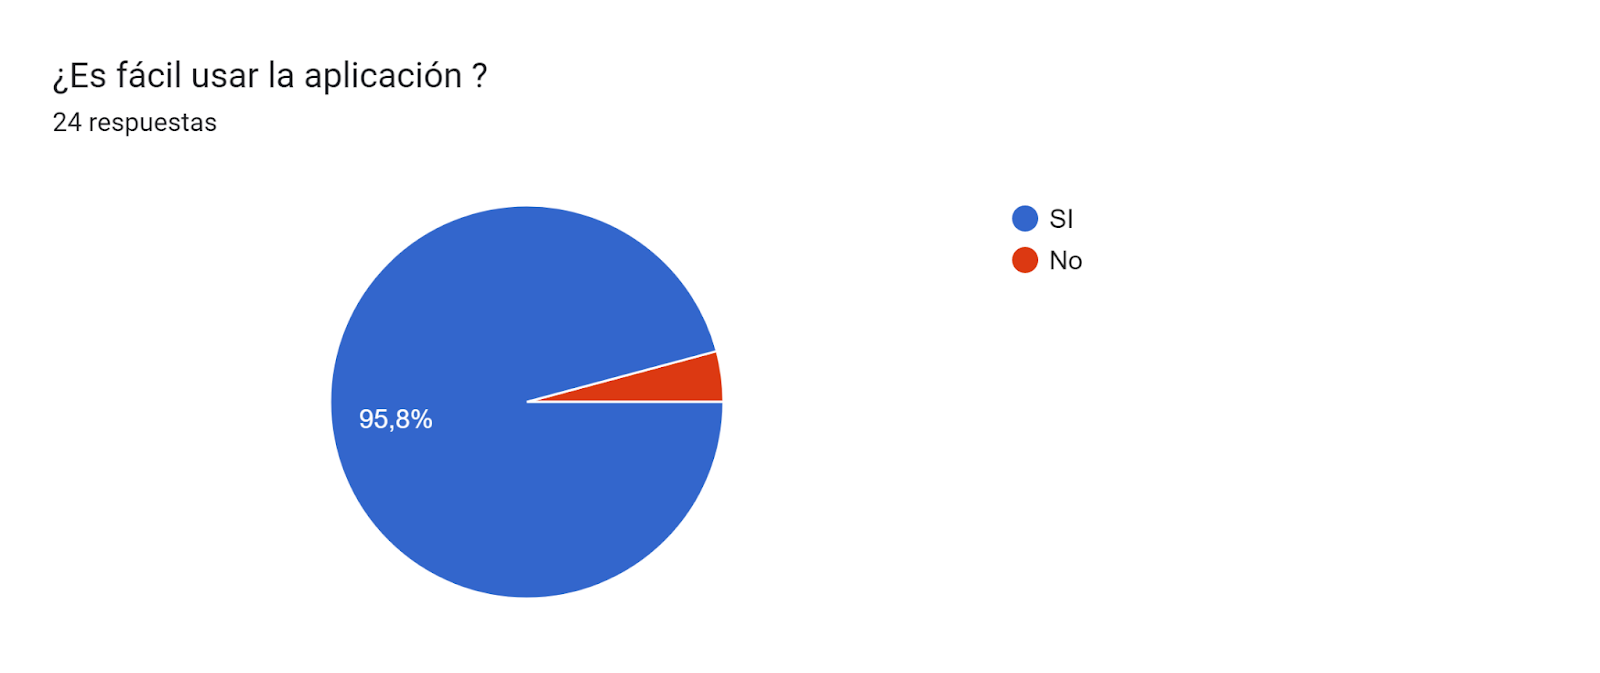
\includegraphics[scale=0.2]{Encuesta1.png}
	\caption{Pregunta sobre facilidad de uso} \textbf{Fuente:} Elaboración propia 
	\label{Encuesta1}
\end{figure}


Al tener varias ventanas con distinta información, es importante saber si a la persona le es fácil llegar a la información, por lo que se usó una escala de 1 -5 como se muestra en la figura \ref{Encuesta2}  donde 1 es difícil y 5 es fácil, el 66.7\% le asignó un valor de 5, el 29.2\% un valor de 4 y el 4.2\% un valor de 3, al sumar el valor de las personas encuestadas que asignaron un valor de 5 - 4, tenemos un 95.8\% que nos permite darlo por válido. 

\begin{figure}[h!]
	\centering
	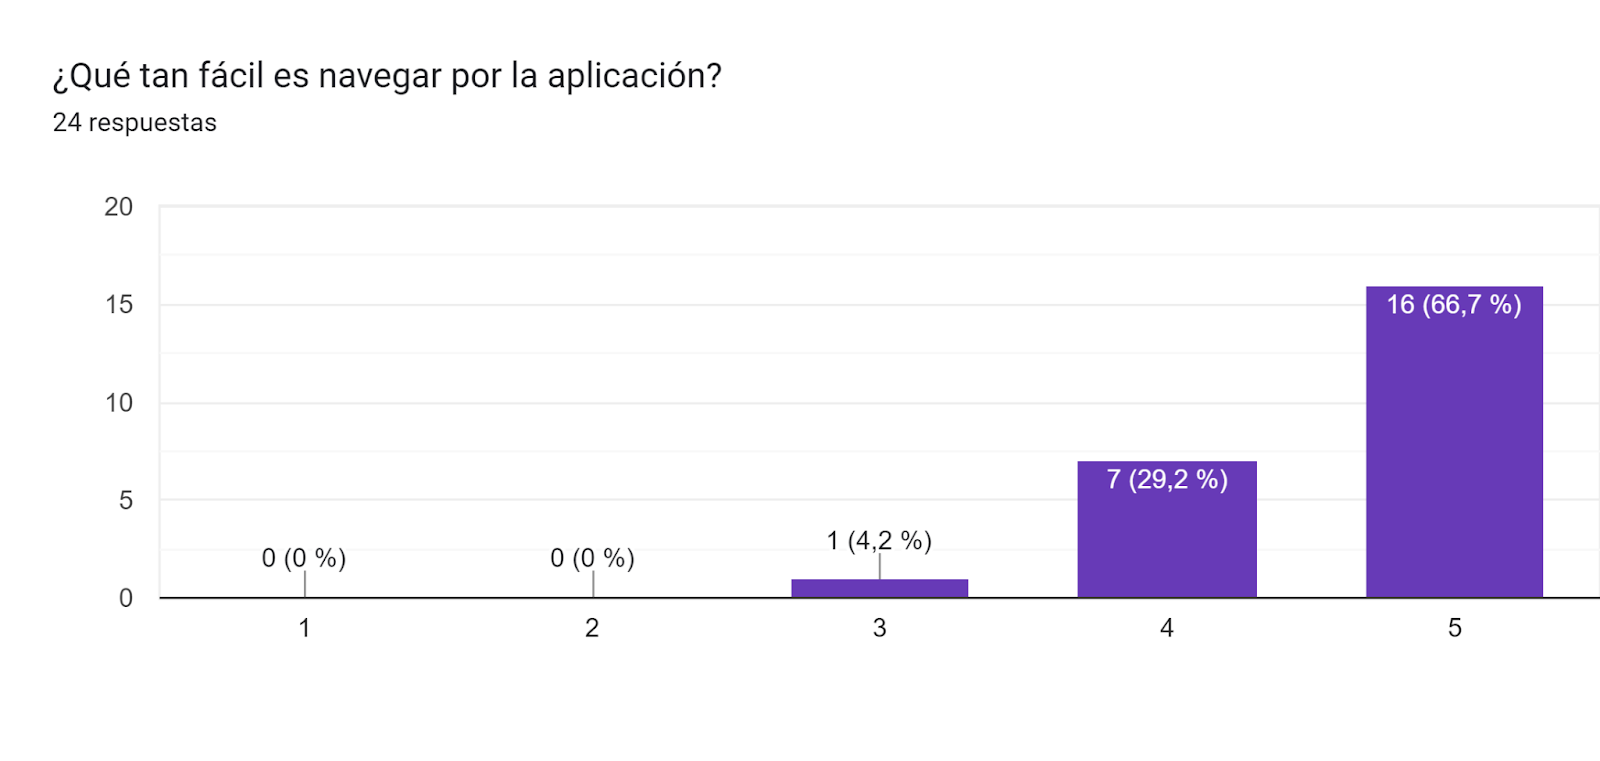
\includegraphics[scale=0.2]{Encuesta2.png}
	\caption{Pregunta sobre facilidad de navegación} \textbf{Referencia: Elaboración propia} 
	\label{Encuesta2}
\end{figure}


Enfocamos una pregunta en la comodidad de la persona al utilizar la aplicación como se muestra en la figura \ref{Encuesta3},  en escala de likert lineal, donde 1 se considera malo y 5 se considera excelente, el 41.7\% de las personas respondieron que fue “excelente”, el 54.2\% respondieron “buena” y el 4.2\% respondió “regular”,  para la validación de esta pregunta el 80\% o más de las personas deben estar ubicadas en las escalas 4-5, de lo cual se obtuvo el 95.8\%.

\begin{figure}[h!]
	\centering
	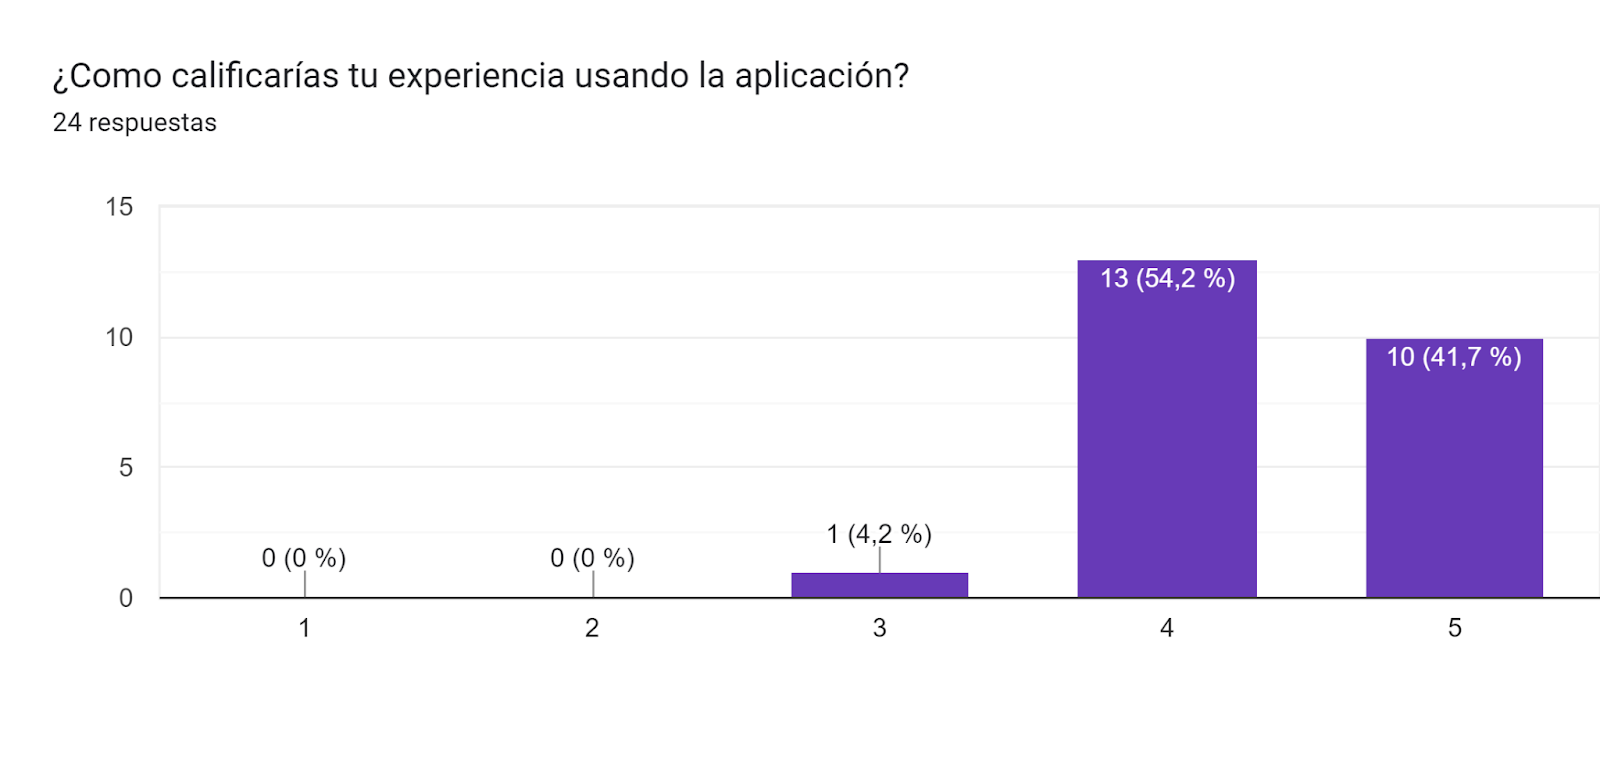
\includegraphics[scale=0.2]{Encuesta3.png}
	\caption{Pregunta sobre la experiencia usando la app} \textbf{Fuente:} Elaboración propia 
	\label{Encuesta3}
\end{figure}

\subsection{Interfaz}

Se formuló también una pregunta, enfocada en que tan visible es la información en tema de colores como se muestra en la figura \ref{Encuesta4} , utilizando un rango de 1 a 5, donde 1 es mala y 5 es buena, el 41.7\% le asignaron un 5, el 54.8\% un 4 y el 12.5\% un 3, para la validación se tenia que más del 80\% se encuentren entre 4 -5 y se obtuvo un 87.5\%.

\begin{figure}[h!]
	\centering
	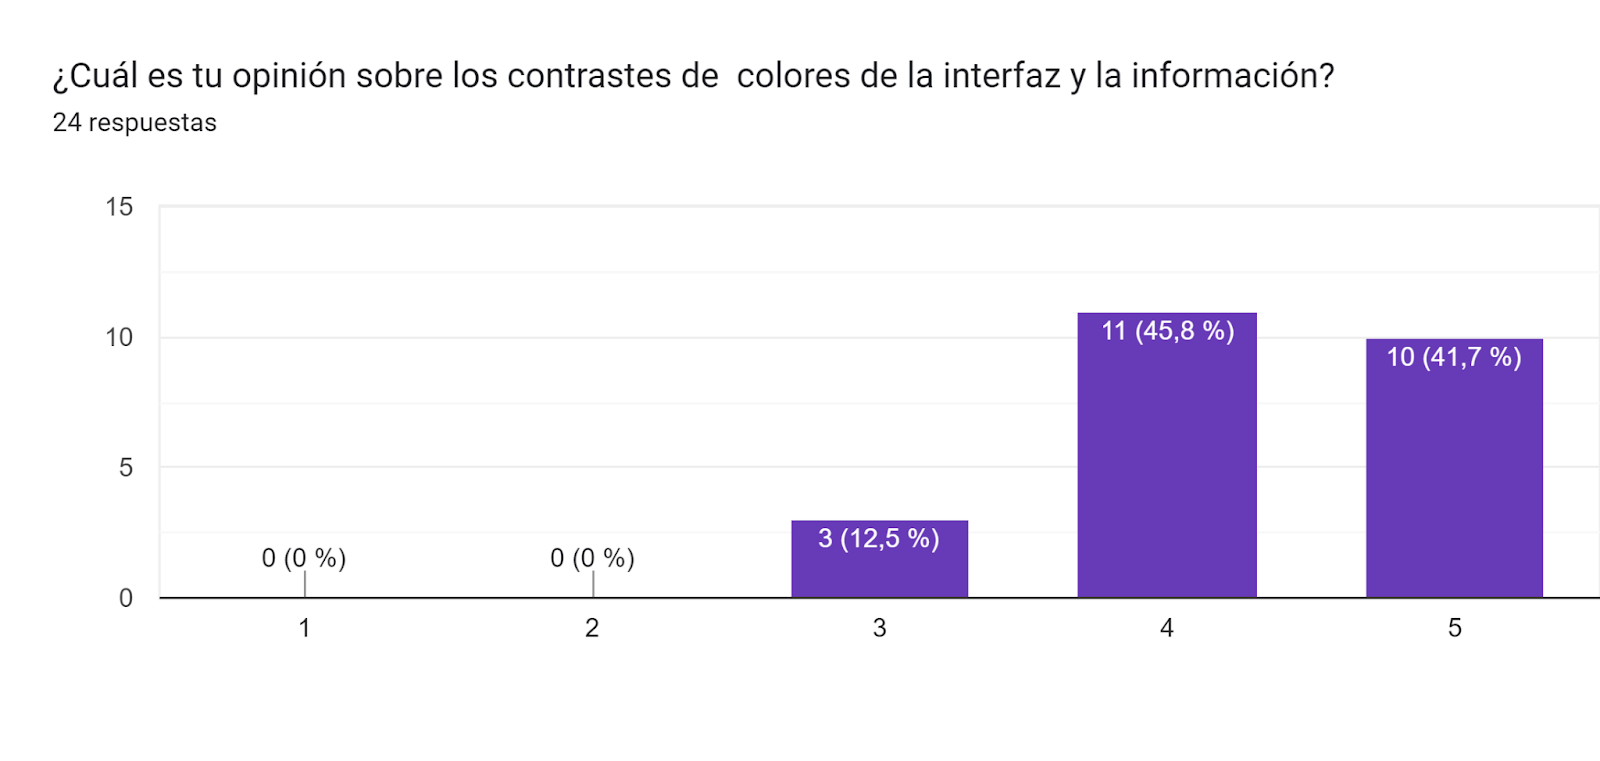
\includegraphics[scale=0.2]{Encuesta4.png}
	\caption{Pregunta sobre colores e información} \textbf{Fuente:} Elaboración propia 
	\label{Encuesta4}
\end{figure}

Al ser una aplicación, en la cual se busca adaptación hacia los distintos dispositivos, se enfoco una pregunta a este tema como se muestra en la figura \ref{Encuesta5}, utilizando un escala de 1 - 5 donde 1 es malo y 5 bueno, el 41.7\% asignaron un valor de 5, el 45.8\% un valor de 4 y el 12.5\% de 3, para validar esta pregunta se establece  un valor de 80\% o más entre 4-5, el total fue de 87.5\%.

\begin{figure}[h!]
	\centering
	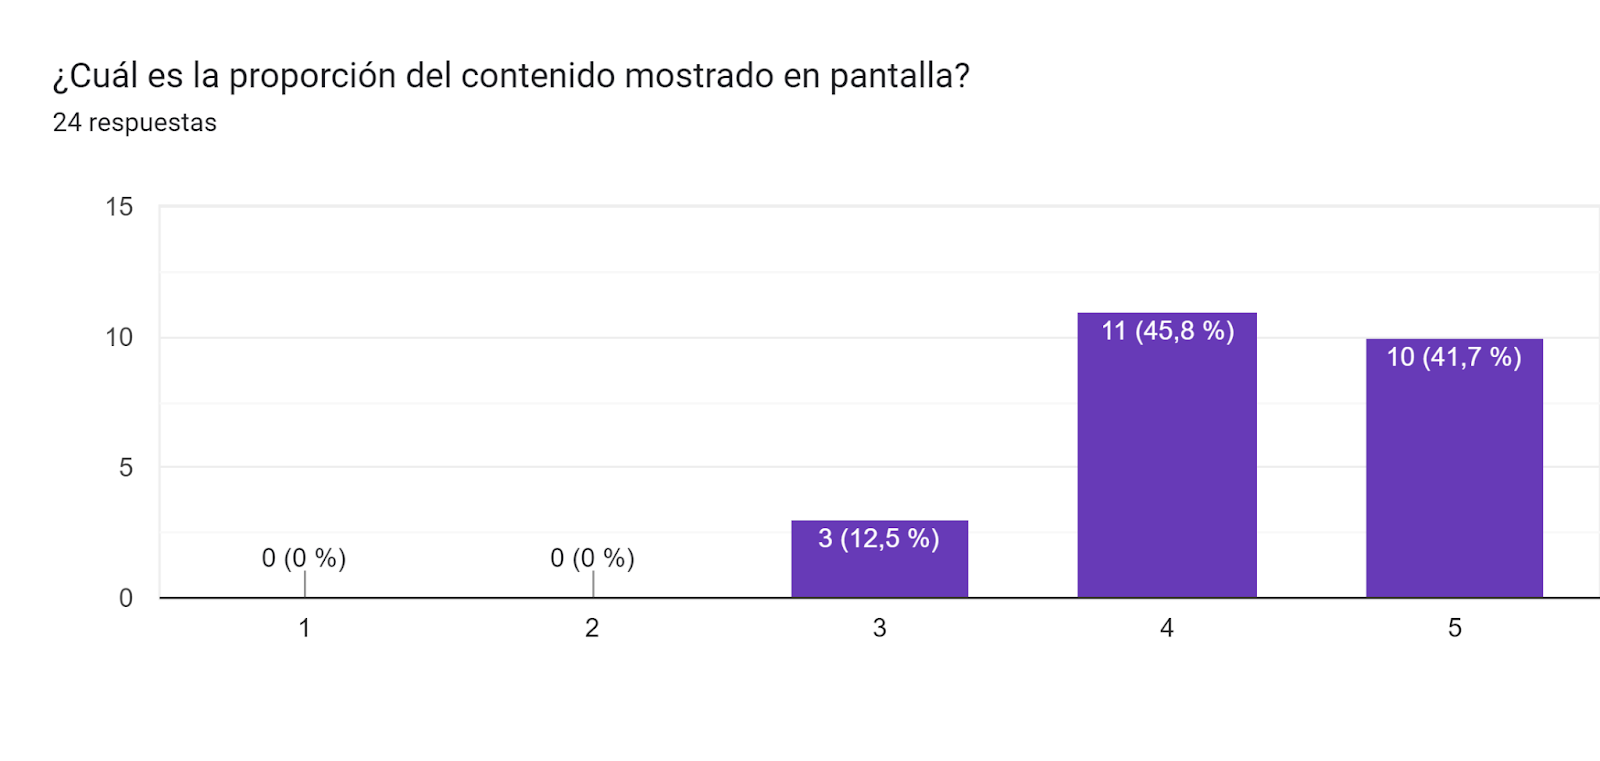
\includegraphics[scale=0.2]{Encuesta5.png}
	\caption{Pregunta proporción de información} \textbf{Fuente:} Elaboración propia 
	\label{Encuesta5}
\end{figure}

\subsection{Sección}

Debido a que se tiene tres secciones principales en la aplicación y estas contienen información valiosa surgen preguntas enfocadas en las mismas, es de resaltar que la sección “General”, es  donde se reproduce el vídeo, “Diámetro”, en el que se muestra el histograma correspondiente al diámetro, “Velocidad”, en la cual se muestra el histograma de velocidad. Para validar se tiene que más del 80\%  es decir 20 personas, hayan opinado entre las opciones muy fácil y fácil o excelente y buena.

Se planteó una pregunta en relación a la accesibilidad como en la figura \ref{Encuesta6} a través de los botones a cada venta, puesto a que no se puede evaluar información a la cual no se pudo acceder, en donde para la sección de “General”, 10 personas lo calificaron como excelente, 13 personas como buena, y 1 personas como regular, para validación se obtuvo 23 personas; para la sección de “Diámetro”, 11 lo calificaron como excelente, 11, como  buena, y 2 como regular, teniendo un valor final de 22 personas que lo validaron; para la sección de “Velocidad”, 10 votaron por excelente, 13 por  buena y 1 personas como regular, teniendo como valor final 23 personas para validación.

\begin{figure}[h!]
	\centering
	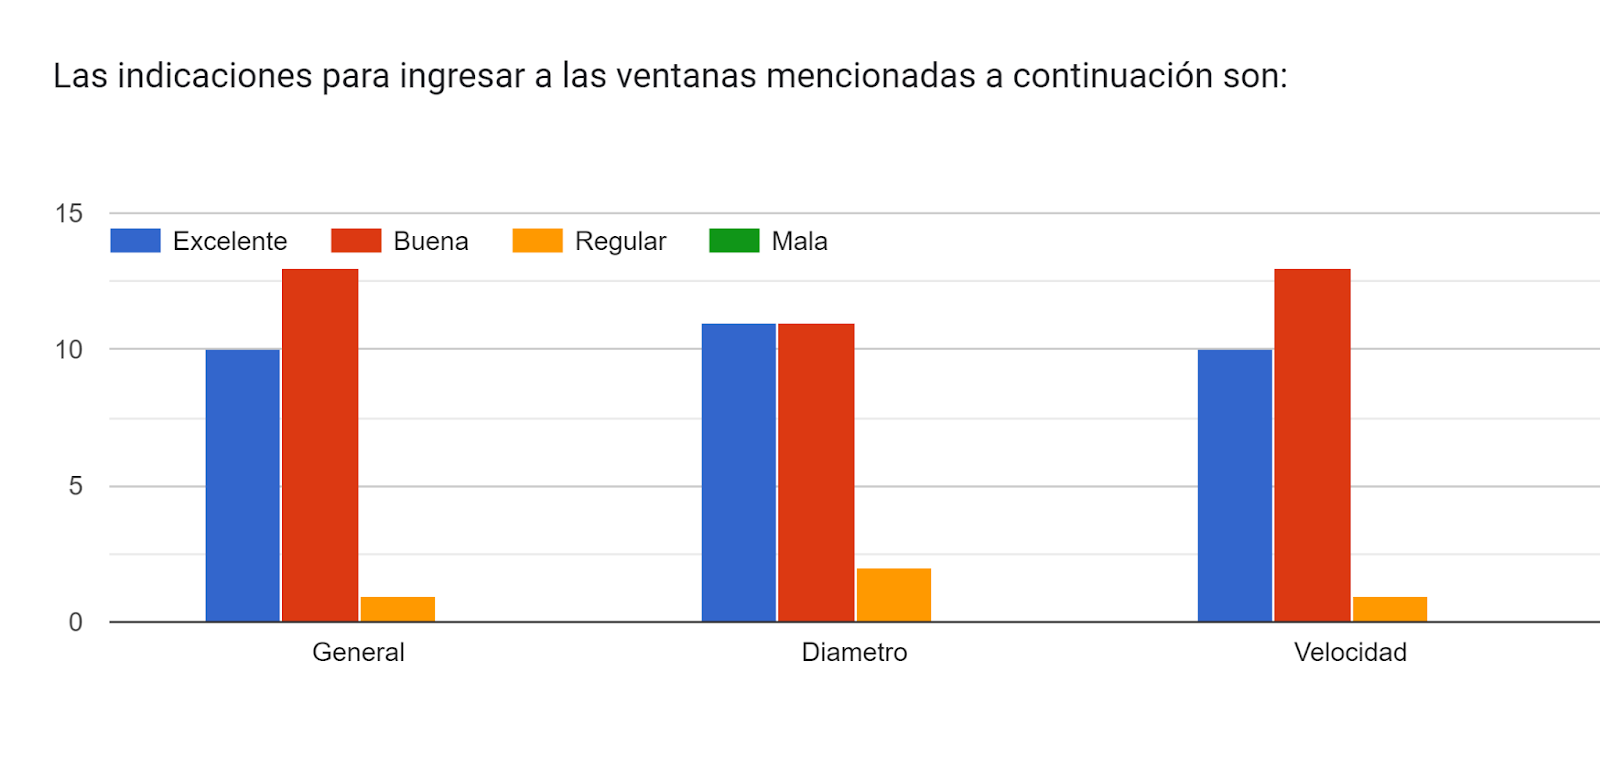
\includegraphics[scale=0.2]{Encuesta6.png}
	\caption{Pregunta indicaciones de ingreso a ventanas} \textbf{Fuente:} Elaboración propia
	\label{Encuesta6}
\end{figure}

Se planteó una pregunta en relación a los textos como en la figura \ref{Encuesta7}, ya que a través de estos se informa sobre el estado del vídeo, así mismo sobre los valores mínimo, máximo y promedio de Diámetro y velocidad, en donde para la sección de “General”, 11 personas lo calificaron como muy Fácil, 10 personas como fácil, y 3 personas como regular, para validación se obtuvo 21 personas; para la sección de “Diámetro”, 9 lo calificaron como muy fácil, 12, como fácil, y 3 como regular, teniendo un valor final de 21 personas que lo validaron; para la sección de “Velocidad”, 9 votaron por muy fácil, 13 por fácil, y 2 por regular, teniendo como valor final 22 personas para validación. 

\begin{figure}[h!]
	\centering
	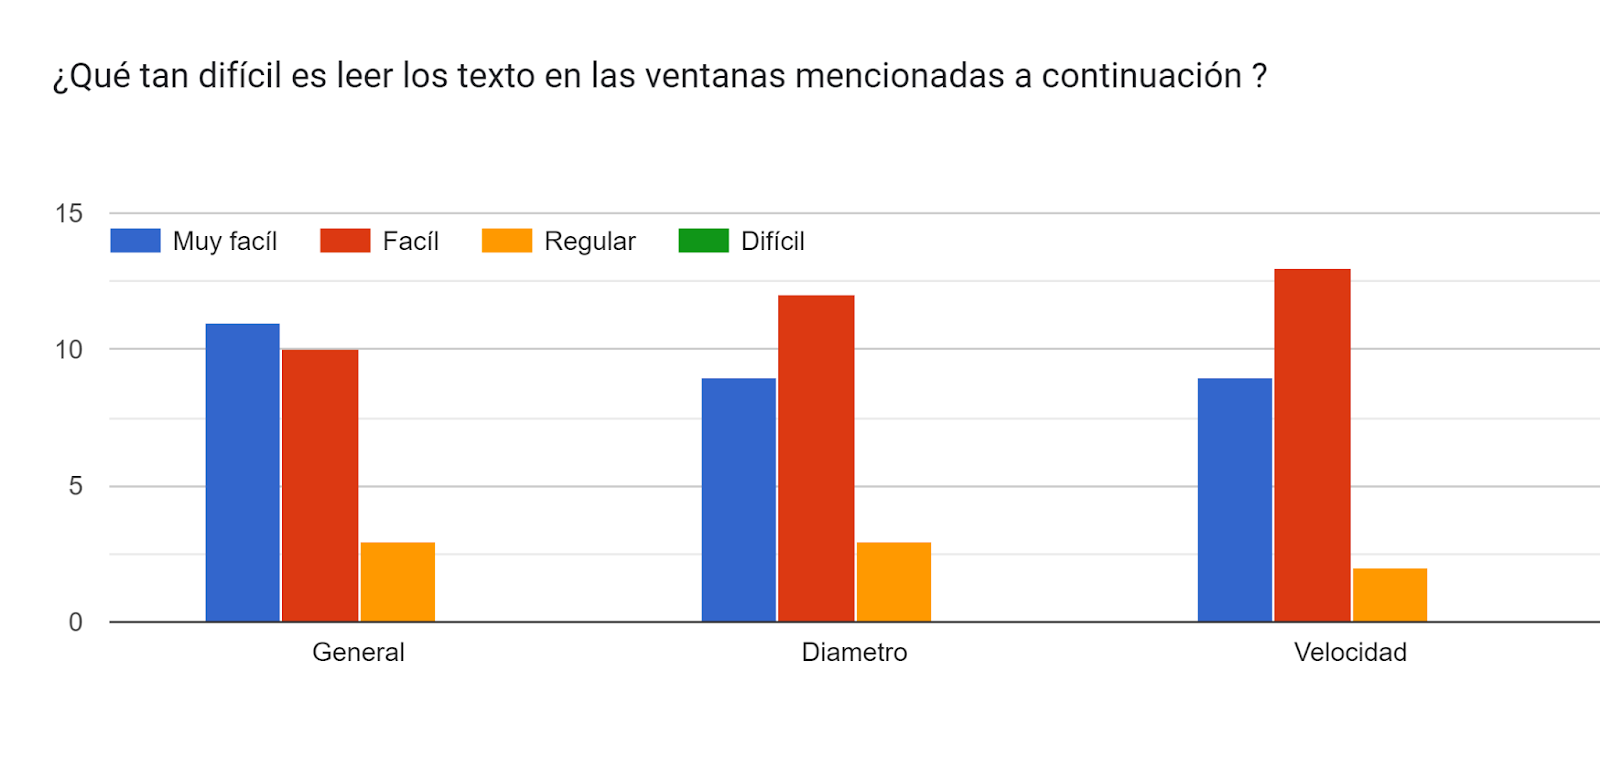
\includegraphics[scale=0.2]{Encuesta7.png}
	\caption{Pregunta sobre dificultad de lectura de textos} \textbf{Fuente:} Elaboración propia
	\label{Encuesta7}
\end{figure} 

Se planteó una pregunta en relación a la relación u organización entre texto, gráficas y botones como en la figura \ref{Encuesta8}, para verificar que toda la información de relevancia se esté mostrando de forma correcta, en donde para la sección de “General”, 12 personas lo calificaron como excelente, 10 personas como buena, y 2 personas como regular, para validación se obtuvo 22 personas; para la sección de “Diámetro”, 10 lo calificaron como excelente, 13 como  buena, y 1 como regular, teniendo un valor final de 23 personas que lo validaron; para la sección de “Velocidad”, 9 votaron por excelente, 15 por  buena, teniendo como valor final 24 personas para validación. 

\begin{figure}[h!]
	\centering
	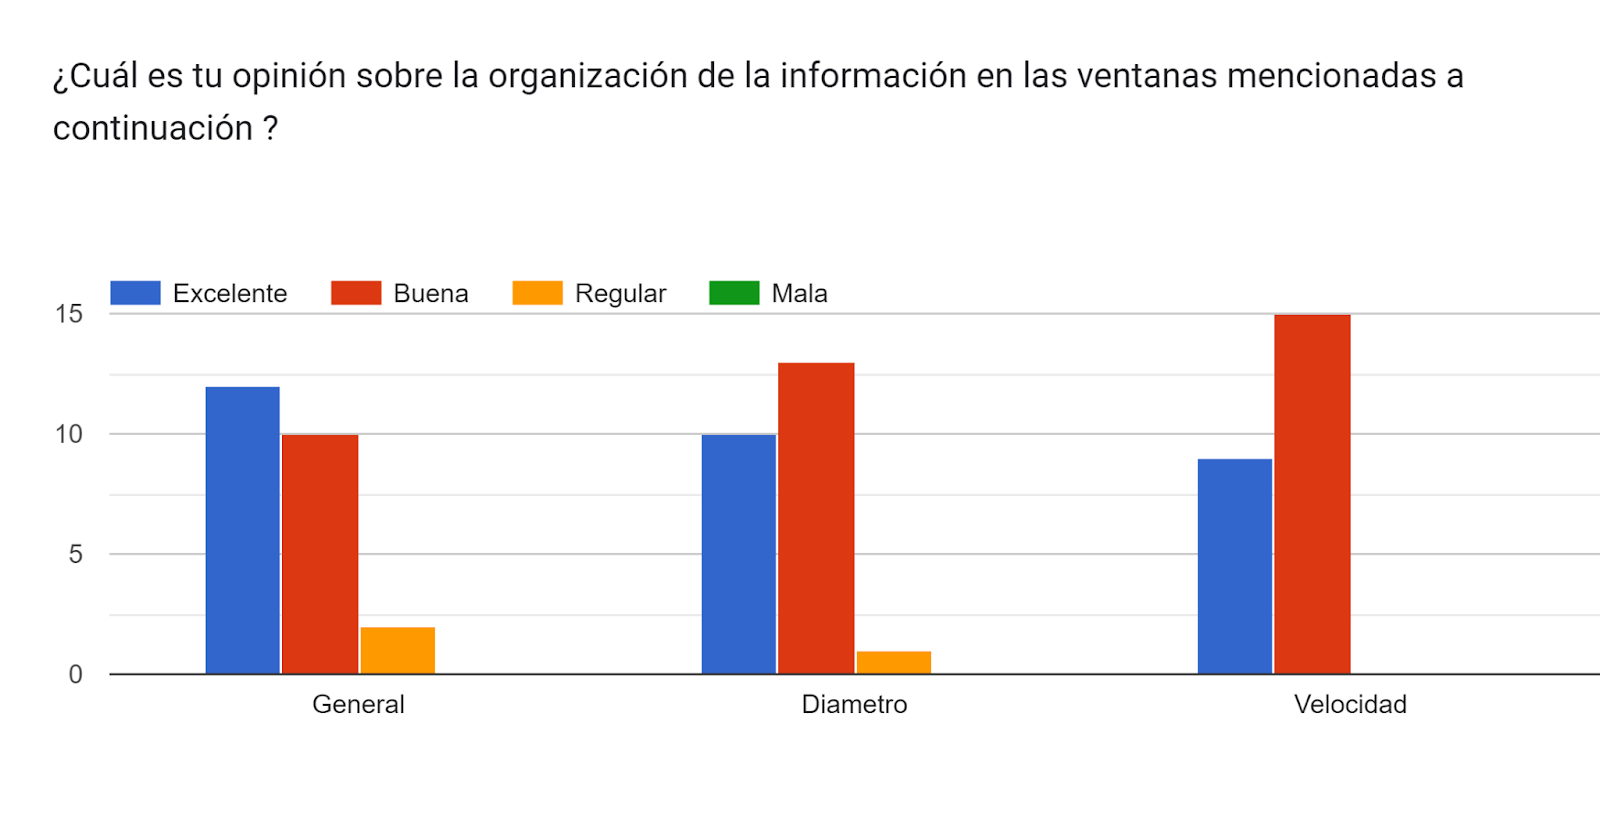
\includegraphics[scale=0.2]{Encuesta8.png}
	\caption{Pregunta de opinión sobre la organizacion de la información } \textbf{Fuente:} Elaboración propia
	\label{Encuesta8}
\end{figure}

Para el caso de la pregunta abierta, fue tipo sugerencias, mejoras o quejas que se tuviera sobre la aplicación, en donde se resaltó, que los colores de la aplicación está bien, pero tratar de hacer más llamativa la aplicación.


\section{Conclusiones }
\begin{itemize}
\item Se logró implementar un sistema de microfotografía con el celular Huawei P30 pro, que cumple la función de  cámara, un “Lente Gran Angular" que realiza la función de microscopio, realizando un mayor zoom sobre el área de trabajo, una lámpara led, como iluminación y un soporte diseñado de forma particular, consiguiendo un acople casi perfecto con el teléfono, brindando seguridad y tomas más precisas; la unión de todos estos elementos, permitió no solo obtener un área de captura de  4.45086 mm2, si no también un sistema que puede ser implementado y adaptado en distintas plantas que hagan uso de la flotación por aire disuelto.
\item Con ayuda de la librería de uso libre OpenCV  y C\#, se desarrolló un algoritmo que utilizando funciones básicas de filtrado, con el propósito de eliminar información no deseada sobre la escena,   también con la función de Hough circules, como método de detección de microburbujas, además de operaciones básicas para el cálculo de velocidad; se puso en funcionamiento un algoritmo con capacidad de detectar microburbujas de tamaños 22$\mu$m a 215 $\mu$m  y velocidades de 2,0966 mm/seg a  21,8404 mm/seg, el algoritmo demostró tener la capacidad de hacer estimaciones de tamaño y velocidad fuera de los límites establecidos, haciendo de este un sistema flexible que puede ser utilizado en pruebas más rigurosas y específicas, haciendo un análisis prácticamente en el tiempo de ejecución del video a procesar.
\item El procesamiento de imágenes demostró ser un medio para caracterización de microburbujas de implementación sencilla puesto a que se necesitan contados recursos para ser empleada y esto sin alterar la planta donde se usa la flotación por aire, presentando un buen desempeño y resultados satisfactorios. Pero este método también presenta algunas notables dificultades, en cuestión de cómo se plantea el cálculo de la velocidad, al ser calculada en un plano 2D el avance de las burbujas hacia el fondo no es apreciado correctamente, e incluso puede alterar el tamaño de algunas burbujas ya que se están alejando del plano focal de captura. En cuestión del tamaño algunas burbujas de gran tamaño las cuales se encuentran al fondo de la zona de captura de imágenes, pueden alterar algunos filtros del procesamiento, lo cual implica que se pueden tener en cuenta burbujas que no se estipulan como válidas según las condiciones de cada proyecto.
\item El software unity, al ser una herramienta multiplataforma, cuyo lenguaje de programación base es C\#, el cual a su vez se puede conectar con OpenCv e implementar diferentes librerías, permite poner en práctica, una aplicación que lleva inmerso un algoritmo capaz de realizar caracterización de microburbujas, que además permite al usuario agregar sus propios videos para caracterizar, siempre que cumplan con las condiciones ya definidas, la interfaz mostrada, lleva al usuario paso a paso, por cada proceso, dejando al final con un resumen gráfico sobre el diámetro y velocidad detectadas, adicional esta aplicación puede operar en dispositivos android los cuales tengan las características mínimas de funcionamiento.
\end{itemize}.

\bibliographystyle{IEEEtran}
\bibliography{Ref}

\section{Anexos}
\begin{table*}[t]
	\begin{tabular}{| c | c | c | c | c | c | c | c |}
	\hline
	
		\multicolumn{8}{ |c| }{\textbf{Primer lote 36 psi}} \\ \hline
	 	\multirow{2}{*}{\textbf{Video}} & \multirow{2}{*}{\textbf{Burbujas}} & \multicolumn{3}{ |c| }{\textbf{Diametro ($\mu$m)}} & \multicolumn{3}{ |c| }{\textbf{Velocidad (mm/s)}} \\
 		&  & \textbf{Minimo} & \textbf{Maximo} & \textbf{Promedio} &\textbf{Minima} & \textbf{Maxima} & \textbf{Promedio}\\ \hline
 	1 & 16 & 22,0147 & 211,3420 & 86,78 & 2,0966 & 14,6563 & 3,57 \\
 	2 & 11 & 35,2236 & 149,7005 & 79,04 & 2,0966 & 10,6365 & 3,64 \\
 	3 & 12 & 35,2236 & 189,3272 & 102.31 & 2,0966 & 14,5087 & 7,11  \\
 	4 & 11 & 26,4177 & 180,5213 & 88.58 & 2,0966 & 2,8017 & 2,11  \\
 	5 & 13 & 35,2236 & 114,4769 & 62,29 & 2,0966 & 4,6051 & 2,2 \\
 	6 & 13 & 30,8207 & 83,6562 & 58,1 & 2,0966 & 2,0966 & 2,1 \\
 	7 & 27 & 26,4177 & 101,2680 & 50,11 & 2,0966 & 16,9476 & 6,04 \\
 	8 & 15 & 22,0147 & 195,9316 & 89.84 & 2,0966 & 11,9172 & 5,13 \\
 	9 & 10 & 22,0147 & 149,7005 & 65.18 & 2,0966 & 9,8784 & 3,68 \\
 	10 & 10 & 22,0147  & 110,0739 & 60.13 & 2,0966 & 4,7312 & 2,55 \\
 	11 & 15 & 30,8207  & 113,0092 & 78.5 & 2,0966  & 2,0966 & 2,1 \\
 	12 & 10 & 44,0295  & 136,4917 & 82.38 & 2,0966  & 10,4066 & 4,06 \\
 	13 & 10 & 30,8207 & 184,9242 & 80.9 & 2,0966 & 12,0557 & 2,9  \\
 	14 & 14 & 22,0147 & 193,7301 & 83.22 & 2,0966 & 8,2364 & 2,33 \\
 	\bottomrule
	\end{tabular}
	\caption{Resultados primer lote 36 psi}
\label{R2}
\end{table*}

\begin{table*}[t]
	\begin{tabular}{| c | c | c | c | c | c | c | c |}
	\hline
	
		\multicolumn{8}{ |c| }{\textbf{Segundo lote 34 psi}} \\ \hline
	 	\multirow{2}{*}{\textbf{Video}} & \multirow{2}{*}{\textbf{Burbujas}} & \multicolumn{3}{ |c| }{\textbf{Diametro ($\mu$m)}} & \multicolumn{3}{ |c| }{\textbf{Velocidad (mm/s)}} \\
 		&  & \textbf{Minimo} & \textbf{Maximo} & \textbf{Promedio} &\textbf{Minima} & \textbf{Maxima} & \textbf{Promedio}\\ \hline
 	1 & 11 & 22,0147 & 189,3272 & 105,88 & 2,0966 & 12,7219 & 2,44 \\
 	2 & 24 & 22,0147 & 211,3420 & 94,22 & 2,0966 & 12,4588 & 5,78 \\
 	3 & 21 & 26,4177 & 184,9242 & 62,95 & 2,0966 & 6,6973 & 2,17  \\
 	4 & 31 & 44,0295 & 193,7301 & 103,09 & 2,0966 & 7,7355 & 2,87  \\
 	5 & 16 & 39,6266 & 193,7301 & 86,83 & 2,0966 & 14,2034 & 3,54 \\
 	6 & 35 & 22,0147 & 167,3124 & 74,96 & 2,0966 & 9,3968 & 3,49 \\
 	7 & 17 & 22,0147 & 211,3420 & 106,96 & 2,0966 & 16,1556 & 3,21  \\
 	8 & 40 & 26,4177 & 206,9390 & 90,18 & 2,0966 & 10,2320 & 2,56 \\
 	9 & 16 & 22,0147 & 198,1331 & 91,17 & 2,0966 & 2,0966 & 2,1 \\
 	10 & 27 & 22,0147  & 180,5213 & 90,57 & 2,0966  & 11,6747 & 2,68 \\
 	11 & 26 & 22,0147  & 211,3420 & 75,57 & 2,0966  & 2,0966 & 2,1 \\
 	12 & 28 & 22,0147  & 180,5213 & 82,42 & 2,0966  & 8,1826 & 2,47 \\
 	13 & 23 & 30,8207 & 215,7449 & 93,23 & 2,0966 & 12,2649 & 2,95 \\
 	\bottomrule
	\end{tabular}
	\caption{Resultados segundo lote 34 psi}
\label{R3}
\end{table*}

\begin{table*}[t]
	\begin{tabular}{| c | c | c | c | c | c | c | c |}
	\hline
	
		\multicolumn{8}{ |c| }{\textbf{Segundo lote 36 psi}} \\ \hline
	 	\multirow{2}{*}{\textbf{Video}} & \multirow{2}{*}{\textbf{Burbujas}} & \multicolumn{3}{ |c| }{\textbf{Diametro ($\mu$m)}} & \multicolumn{3}{ |c| }{\textbf{Velocidad (mm/s)}} \\
 		&  & \textbf{Minimo} & \textbf{Maximo} & \textbf{Promedio} &\textbf{Minima} & \textbf{Maxima} & \textbf{Promedio}\\ \hline
 	1 & 18 & 22,0147 & 162,9094 & 88,69 & 2,0966 & 12,8390 & 3,03 \\
 	2 & 29 & 35,2236 & 215,7449 & 92,27 & 2,0966 & 7,4193& 2,52 \\
 	3 & 38 & 22,0147 & 165,8447 & 77,95 & 2,0966 & 11,3939 & 4,53  \\
 	4 & 20 & 22,0147 & 206,9390 & 91,69 & 2,0966 & 6,5507 & 2,35  \\
 	5 & 24 & 26,4177 & 206,9390 & 91,65 & 2,0966 & 12,9895 & 3,51 \\
 	6 & 35 & 22,0147 & 167,3124 & 74,96 & 2,0966 & 9,3968 & 3,49 \\
 	7 & 19 & 22,0147 & 198,1331 & 63,1 & 2,0966 & 8,1193 & 2,26  \\
 	8 & 16 & 30,8207 & 202,5361 & 98,15 & 2,0966 & 14,3450 & 4,77 \\
 	9 & 25 & 22,0147 & 149,7005 & 59,89 & 2,0966 & 13,1504 & 4,46 \\
 	10 & 11 & 35,2236  & 132,0887 & 73,81 & 2,0966  & 13,7998 & 5,08 \\
 	11 & 22 & 22,0147  & 198,1331 & 74,9 & 2,0966  & 8,9282 & 3,39 \\
 	12 & 28 & 33,0221  & 198,1331 & 71,5 & 2,0966  & 21,8404 & 7,18 \\
 	\bottomrule
	\end{tabular}
	\caption{Resultados segundo lote 36 psi}
\label{R4}
\end{table*}

\begin{table*}[t]
	\centering
	\begin{tabular}{| c | c | c | c | c | c |}
	\toprule	
		\multicolumn{6}{ |c| }{\textbf{ESPECIFICACIONES TELÉFONOS}} \\ \hline
	 	 \textbf{RAM} & \textbf{ANDROID} & \textbf{PROCESADOR}  & \textbf{SIRVE}  & \textbf{FLUIDEZ} &   \textbf{CANT.}  \\
	 	\midrule
    	2 GB & 7.1.1 & Qualcomm Snapdragon 410 & No & -  & 1 \\
    	3 GB & 10 & Octa Core Helio P 23 & Si & Baja & 3 \\
    	2 GB & 7.0.1 & Qualcomm Snapdragon 617 & No & - & 1 \\
    	4 GB & 11 & Qualcomm Snapdragon 662 & Si & Buena & 3 \\
    	4 GB & 10.1 & Huawei Kirin 710 F & Si & Baja & 2\\
    	4 GB & 9 & Octa core Max & Si & Buena  & 1\\
    	8 GB & 12 & Octa core Max & Si & Buena & 2 \\
    	5 GB & 11 & Qualcomm Snapdragon 680 & Si & Buena & 5\\
    	4 GB & 12 & Octa-Core Max & Si & Buena & 3 \\
    	1 GB & 5.1.1 & Quad-core  & No & -  & 1\\
    	4 GB & 12 & Helio G35 Octa core  & No & - & 1 \\
    	6 GB & 10 & Huawei Kirin 980 & Si & Buena & 1\\
    	
    \bottomrule
    \end{tabular}
	\caption{Datos teléfonos probados}
	\label{TablaCEL}
\end{table*}


\end{document}
